\documentclass[11pt,]{article}
\usepackage[margin=1in]{geometry}
\newcommand*{\authorfont}{\fontfamily{phv}\selectfont}
\usepackage[]{mathpazo}

\usepackage{amssymb,amsmath}
\usepackage{xcolor}

%TIKZ and Flow chart material
\usepackage{tikz}
\usetikzlibrary{shapes.geometric, arrows}
\tikzstyle{startstop} = [rectangle, rounded corners, minimum width=3cm, minimum height=1cm,text centered, draw=black, fill=red!30]
\tikzstyle{io} = [trapezium, trapezium left angle=70, trapezium right angle=110, minimum width=3cm, minimum height=1cm, text centered, draw=black,fill=white]
\tikzstyle{process} = [rectangle, minimum width=3cm, minimum height=1cm, text centered, draw=black, fill=white]
\tikzstyle{decision} = [diamond, minimum width=3cm, minimum height=1cm, text centered, draw=black, fill=white]
\tikzstyle{smalldecision} = [diamond, minimum width=1cm, minimum height=1cm, text centered, draw=black, fill=white]
\tikzstyle{arrow} = [thick,->,>=stealth]
\tikzstyle{line} = [thick,-]
\tikzstyle{dot} = [circle,inner sep=0.5pt,draw=black, fill=black]


%\tikzstyle{startstop} = [rectangle, rounded corners, minimum width=3cm, minimum height=1cm,text centered, %draw=black, fill=red!30]
%\tikzstyle{io} = [trapezium, trapezium left angle=70, trapezium right angle=110, minimum width=3cm, %minimum height=1cm, text centered, draw=black,fill=white]
%\tikzstyle{process} = [rectangle, minimum width=3cm, minimum height=1cm, text centered, draw=black, %fill=white]
%\tikzstyle{decision} = [diamond, minimum width=3cm, minimum height=1cm, text centered, draw=black, %fill=green!30]
%\tikzstyle{arrow} = [thick,->,>=stealth]




\usepackage{abstract}
\renewcommand{\abstractname}{}    % clear the title
\renewcommand{\absnamepos}{empty} % originally center
\newcommand{\blankline}{\quad\pagebreak[2]}

\providecommand{\tightlist}{%
  \setlength{\itemsep}{0pt}\setlength{\parskip}{0pt}}
\usepackage{longtable,booktabs}

\usepackage{parskip}
\usepackage{titlesec}
\titlespacing\section{0pt}{12pt plus 4pt minus 2pt}{6pt plus 2pt minus 2pt}
\titlespacing\subsection{0pt}{12pt plus 4pt minus 2pt}{6pt plus 2pt minus 2pt}

\titleformat*{\subsubsection}{\normalsize\itshape}

\usepackage{titling}
\setlength{\droptitle}{-.25cm}

%\setlength{\parindent}{0pt}
%\setlength{\parskip}{6pt plus 2pt minus 1pt}
%\setlength{\emergencystretch}{3em}  % prevent overfull lines

\usepackage[T1]{fontenc}
\usepackage[utf8]{inputenc}

\usepackage{fancyhdr}
\pagestyle{fancy}
\usepackage{lastpage}
\renewcommand{\headrulewidth}{0.3pt}
\renewcommand{\footrulewidth}{0.0pt}
%\lhead{\footnotesize Problem Set \#7 }
\lhead{\footnotesize BUEC 311: Problem Set \#7, Firm Theory and Perfect
Competition}
\rhead{\footnotesize \today}
\lfoot{\small \copyright }
\cfoot{}
\rfoot{\small \thepage/\pageref*{LastPage}}

\fancypagestyle{firststyle}
{
\renewcommand{\headrulewidth}{0pt}%
   \fancyhf{}
   \fancyfoot[C]{\thepage/\pageref*{LastPage}}
}

%\def\labelitemi{--}
%\usepackage{enumitem}
%\setitemize[0]{leftmargin=25pt}
%\setenumerate[0]{leftmargin=25pt}




\makeatletter
\@ifpackageloaded{hyperref}{}{%
\ifxetex
  \usepackage[setpagesize=false, % page size defined by xetex
              unicode=false, % unicode breaks when used with xetex
              xetex]{hyperref}
\else
  \usepackage[unicode=true]{hyperref}
\fi
}
\@ifpackageloaded{color}{
    \PassOptionsToPackage{usenames,dvipsnames}{color}
}{%
    \usepackage[usenames,dvipsnames]{color}
}
\makeatother
\hypersetup{breaklinks=true,
            bookmarks=true,
            pdfauthor={},
             pdfkeywords = {},
            pdftitle={Problem Set \#7: Firm Theory and Perfect
Competition},
            colorlinks=true,
            citecolor=blue,
            urlcolor=blue,
            linkcolor=magenta,
            pdfborder={0 0 0}}
\urlstyle{same}  % don't use monospace font for urls


\setcounter{secnumdepth}{0}


%



\usepackage{setspace}

\title{\vspace{-1.5cm}\Large{BUEC 311: Business Economics, Organization
and Management}\medskip\\\Large{Problem Set \#7}
\medskip\\\Large{Firm Theory and Perfect Competition}
}
\date{\vspace{-.75cm}\Large{\today}}

\definecolor{light-gray}{gray}{0.8}


\begin{document}

\vspace{-5cm}\maketitle
 \tikz [remember picture,overlay]
    %\node[yshift=-1.65cm,xshift=0cm] at (current page.north)
    %\node[yshift=-1.65cm,xshift=0cm] at (current page.north)
        %or: (current page.center)
        \node[yshift=-1cm,xshift=6.5cm] at (current page.north west)
        %{
\includegraphics[width=3in]{UA-ASB-COLOUR.png}};
        {
\includegraphics[width=.5\paperwidth]{../images/UA-ASB-COLOUR.png}};
\vspace{-.75cm}		
		\thispagestyle{firststyle}



Single Answer

\begin{enumerate}
\def\labelenumi{\arabic{enumi})}
\tightlist
\item
  A \_\_\_\_\_\_\_\_ is a governance structure where owners are not
  personally liable.
\end{enumerate}

\begin{enumerate}
\def\labelenumi{\Alph{enumi})}
\tightlist
\item
  sole proprietorship
\item
  partnership
\item
  mixed enterprise
\item
  corporation
\end{enumerate}

Answer: D

\begin{enumerate}
\def\labelenumi{\arabic{enumi})}
\setcounter{enumi}{1}
\tightlist
\item
  Economists typically assume that the owners of firms wish to
\end{enumerate}

\begin{enumerate}
\def\labelenumi{\Alph{enumi})}
\tightlist
\item
  produce efficiently.
\item
  maximize sales revenues.
\item
  maximize profits.
\item
  All of the above.
\end{enumerate}

Answer: C

\begin{enumerate}
\def\labelenumi{\arabic{enumi})}
\setcounter{enumi}{2}
\tightlist
\item
  A small business owner earns \$50,000 in revenue annually. The
  explicit annual costs equal \$30,000. The owner could work for someone
  else and earn \$25,000 annually. The owner's accountant would likely
  measure profit as \_\_\_\_\_\_\_\_ but an economic assessment would
  estimate a profit of \_\_\_\_\_\_\_\_.
\end{enumerate}

\begin{enumerate}
\def\labelenumi{\Alph{enumi})}
\tightlist
\item
  \$20,000, \$20,000
\item
  \$20,000, -\$5,000
\item
  \$25,000, -\$5,000
\item
  \$25,000, \$20,000
\end{enumerate}

Answer: B

\begin{enumerate}
\def\labelenumi{\arabic{enumi})}
\setcounter{enumi}{3}
\tightlist
\item
  A firm optimally sets its output where
\end{enumerate}

\begin{enumerate}
\def\labelenumi{\Alph{enumi})}
\tightlist
\item
  marginal profit is zero.
\item
  marginal revenue is maximized.
\item
  marginal profit equals marginal revenue.
\item
  marginal profit is maximized.
\end{enumerate}

Answer: A

\begin{enumerate}
\def\labelenumi{\arabic{enumi})}
\setcounter{enumi}{4}
\tightlist
\item
  If marginal revenue equals marginal cost, the firm is maximizing
  profits as long as
\end{enumerate}

\begin{enumerate}
\def\labelenumi{\Alph{enumi})}
\tightlist
\item
  the resulting profits are positive.
\item
  marginal cost exceeds marginal revenue for greater levels of output.
\item
  the average cost curve lies above the demand curve.
\item
  All of the above are required.
\end{enumerate}

Answer: B

\begin{center}
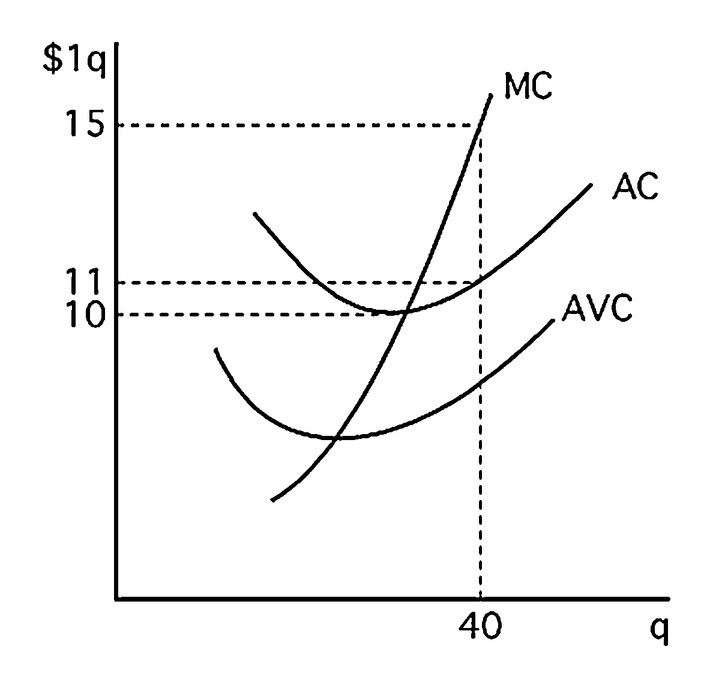
\includegraphics[width=0.65\textwidth]{week_11.jpg}
\end{center}

\begin{enumerate}
\def\labelenumi{\arabic{enumi})}
\setcounter{enumi}{5}
\tightlist
\item
  The above figure shows the cost curves for a competitive firm. If the
  firm is to earn economic profit, price must exceed
\end{enumerate}

\begin{enumerate}
\def\labelenumi{\Alph{enumi})}
\tightlist
\item
  \$0.
\item
  \$5.
\item
  \$10.
\item
  \$11.
\end{enumerate}

Answer: C

\begin{enumerate}
\def\labelenumi{\arabic{enumi})}
\setcounter{enumi}{6}
\tightlist
\item
  Using the above figure which shows the cost curves for a competitive
  firm, you can conclude that the firm should shut down in the short run
  if the price is equal to any number below:
\end{enumerate}

\begin{enumerate}
\def\labelenumi{\Alph{enumi})}
\tightlist
\item
  \$15.
\item
  \$10.
\item
  \$11
\item
  None of the above
\end{enumerate}

Answer: D

\begin{enumerate}
\def\labelenumi{\arabic{enumi})}
\setcounter{enumi}{7}
\tightlist
\item
  If a competitive firm maximizes short-run profits by producing some
  quantity of output, which of the following must be TRUE at that level
  of output?
\end{enumerate}

\begin{enumerate}
\def\labelenumi{\Alph{enumi})}
\tightlist
\item
  p = MC
\item
  MR = MC
\item
  p \(\geq\) AVC
\item
  All of the above.
\end{enumerate}

Answer: D

\begin{enumerate}
\def\labelenumi{\arabic{enumi})}
\setcounter{enumi}{8}
\tightlist
\item
  If a profit-maximizing firm finds that, at its current level of
  production, MR\textless MC, it will
\end{enumerate}

\begin{enumerate}
\def\labelenumi{\Alph{enumi})}
\tightlist
\item
  decrease output.
\item
  increase output.
\item
  shut down.
\item
  operate at a loss.
\end{enumerate}

Answer: A

\begin{enumerate}
\def\labelenumi{\arabic{enumi})}
\setcounter{enumi}{9}
\tightlist
\item
  True or false: If a firm sets marginal revenue equal to marginal cost
  it will make an economic profit.
\end{enumerate}

Answer: False. When a firm sets MR = MC it maximizes profits, but the
profit-maximizing level of output might still be negative (the smallest
loss possible).

\begin{enumerate}
\def\labelenumi{\arabic{enumi})}
\setcounter{enumi}{10}
\tightlist
\item
  Economists define a market to be competitive when the firms
\end{enumerate}

\begin{enumerate}
\def\labelenumi{\Alph{enumi})}
\tightlist
\item
  spend large amounts of money on advertising to lure customers away
  from the competition.
\item
  watch each other's behavior closely.
\item
  are price takers.
\item
  All of the above.
\end{enumerate}

Answer: C

\begin{enumerate}
\def\labelenumi{\arabic{enumi})}
\setcounter{enumi}{11}
\tightlist
\item
  Firms that exhibit price-taking behavior
\end{enumerate}

\begin{enumerate}
\def\labelenumi{\Alph{enumi})}
\tightlist
\item
  wait for other firms to set price, take it as given, and charge a
  higher price.
\item
  have outputs that are too small to influence market price and thus
  take it as given.
\item
  take pricing behavior in their own hands.
\item
  are independently capable of setting price.
\end{enumerate}

Answer: B

\begin{enumerate}
\def\labelenumi{\arabic{enumi})}
\setcounter{enumi}{12}
\tightlist
\item
  In a perfectly competitive market
\end{enumerate}

\begin{enumerate}
\def\labelenumi{\Alph{enumi})}
\tightlist
\item
  firms can freely enter and exit.
\item
  firms sell a differentiated product.
\item
  transaction costs are high.
\item
  All of the above.
\end{enumerate}

Answer: A

\begin{enumerate}
\def\labelenumi{\arabic{enumi})}
\setcounter{enumi}{13}
\tightlist
\item
  In a perfectly competitive market
\end{enumerate}

\begin{enumerate}
\def\labelenumi{\Alph{enumi})}
\tightlist
\item
  buyers are price-takers.
\item
  buyers view products from different firms as differentiated.
\item
  individual buyers have horizontal demand curves.
\item
  firms' demand curves are vertical.
\end{enumerate}

Answer: A

\begin{enumerate}
\def\labelenumi{\arabic{enumi})}
\setcounter{enumi}{14}
\tightlist
\item
  The economist's definition of the short run is
\end{enumerate}

\begin{enumerate}
\def\labelenumi{\Alph{enumi})}
\tightlist
\item
  usually 3-6 months.
\item
  when at least one of the firm's input choices are fixed
\item
  when a firm has to decide whether or not to exit.
\item
  identical to the long run for most firms.
\item
  All of the above
\end{enumerate}

Answer: B

\begin{enumerate}
\def\labelenumi{\arabic{enumi})}
\setcounter{enumi}{15}
\tightlist
\item
  In the short run
\end{enumerate}

\begin{enumerate}
\def\labelenumi{\Alph{enumi})}
\tightlist
\item
  firms will shut down if operating at a loss.
\item
  profit maximizing firms have identical short run supply curves.
\item
  firms may choose to operate at a loss.
\item
  most firms have short run supply curves that are the same as their
  long run supply curves.
\end{enumerate}

Answer: C

\begin{enumerate}
\def\labelenumi{\arabic{enumi})}
\setcounter{enumi}{15}
\tightlist
\item
  In the long run
\end{enumerate}

\begin{enumerate}
\def\labelenumi{\Alph{enumi})}
\tightlist
\item
  firms will shut down if operating at a loss.
\item
  profit maximizing firms have identical supply curves.
\item
  firms may choose to operate at a loss.
\item
  most firms have supply curves that are the same as their long run
  average cost curves.
\item
  all of the above Answer: A
\end{enumerate}

\begin{enumerate}
\def\labelenumi{\arabic{enumi})}
\setcounter{enumi}{16}
\tightlist
\item
  If a competitive firm finds that it maximizes short-run profits by
  shutting down, which of the following must be TRUE?
\end{enumerate}

\begin{enumerate}
\def\labelenumi{\Alph{enumi})}
\tightlist
\item
  p \textless{} AVC for all levels of output.
\item
  p \textless{} AVC only for the level of output at which p = MC.
\item
  p \textless{} AVC only if the firm has no fixed costs.
\item
  The firm will earn zero profit. Answer: A
\end{enumerate}

\begin{enumerate}
\def\labelenumi{\arabic{enumi})}
\setcounter{enumi}{17}
\tightlist
\item
  The competitive firm's supply curve is equal to
\end{enumerate}

\begin{enumerate}
\def\labelenumi{\Alph{enumi})}
\tightlist
\item
  its marginal cost curve.
\item
  the portion of its marginal cost curve that lies above AC.
\item
  the portion of its marginal cost curve that lies above AVC.
\item
  the portion of its marginal cost curve that lies above AFC. Answer: C
\end{enumerate}

\begin{enumerate}
\def\labelenumi{\arabic{enumi})}
\setcounter{enumi}{18}
\tightlist
\item
  In the long run, profits will equal zero in a competitive market
  because of
\end{enumerate}

\begin{enumerate}
\def\labelenumi{\Alph{enumi})}
\tightlist
\item
  constant returns to scale.
\item
  identical products being produced by all firms.
\item
  the availability of information.
\item
  free entry and exit. Answer: D, although you'd win an argument if you
  said that this only holds with identical firms
\end{enumerate}

\begin{enumerate}
\def\labelenumi{\arabic{enumi})}
\setcounter{enumi}{19}
\tightlist
\item
  A firm will enter a competitive market when
\end{enumerate}

\begin{enumerate}
\def\labelenumi{\Alph{enumi})}
\tightlist
\item
  it can gather market share at the expense of incumbent firms.
\item
  it would not be the last firm entering.
\item
  it can earn a positive long-run profit.
\item
  the long-run supply curve is upward sloping. Answer: C
\end{enumerate}




\end{document}
